% !TeX root = ../main.tex
\chapter{绪论}

\section{研究的背景和意义}


数据中心是互联网的 ``大脑'',也是人类存储海量数据、进行大规模计算和提供互联网服务的基础设施。21 世纪第一个十年,数据中心主要处理 Web 网站、搜索引擎等容易并行的任务;通用处理器的高速性能提升也使得专用硬件的优势不甚明显。因此,互联网数据中心多使用大量低成本的标准服务器搭建。

近十年来,大数据与人工智能的兴起改变了数据中心的应用负载特性。一方面,大数据处理、机器学习等负载对算力要求很高。然而,由于摩尔定律的放缓和 Dennard 缩放定律的终结,近十年来,通用处理器的频率提升和多核核数增加都受到功耗墙的限制。因此,通用处理器性能提升 ``免费的午餐'' 已经结束,体系结构的创新迎来了春天,GPU、FPGA、TPU 等定制化硬件在数据中心内大量部署。另一方面,大数据处理、机器学习等负载需要多个节点紧密协同处理,对节点间的通信带宽和延迟要求较高。因此,近十年来,数据中心网络从 1 Gbps 发展到 40 Gbps,并有向 100 Gbps 演进的趋势。定制化硬件之间的专用互连也成为趋势。因此,如英伟达 CEO 黄仁勋所说,未来的数据中心会像超级计算机一样 \cite{nvidia-datacenter}。

与此同时,数据中心的运营模式也在经历一场云化的变革。数据中心的算力逐渐集中到少数几家云厂商,每家拥有数以百万计的服务器。由于云数据中心的规模大,云服务商一方面有足够的规模来平摊服务器、板卡甚至芯片的设计和流片成本,另一方面通过软件优化也可以提高性能指标、降低成本,获得可观的经济效益。由于上述应用负载特性的转变和数据中心的云化,工程师获得了从硬件、系统软件到应用的全栈优化机会。

在云数据中心中,不同的租户共享一个巨大的计算、存储和网络资源池。为了实现资源共享和性能隔离,数据中心需要实现计算、存储和网络的虚拟化。如图 \ref{intro:fig:virt-architecture} 所示,在基础设施作为服务(IaaS)的云服务模式下,计算节点上需要提供虚拟网络、虚拟云存储、虚拟本地存储等服务,实际的网络和云存储资源则位于独立的网络节点和存储节点上。计算节点上的虚拟网络和存储服务把数据中心内物理上分散的网络和存储资源虚拟化成逻辑上统一的资源(``多虚一'')。网络和存储节点则不仅需要把物理资源共享给多个计算节点上不同租户的虚拟机使用(``一虚多''),还需要提供数据处理功能和高层抽象。网络节点需要提供防火墙、负载均衡、加密隧道网关、网络地址转换(NAT)等网络功能;存储节点需要进行数据结构处理以提供对象存储、文件系统存储等高层抽象,还需要进行复制(replication)以实现容灾。


\begin{figure}[htbp]
	\centering
	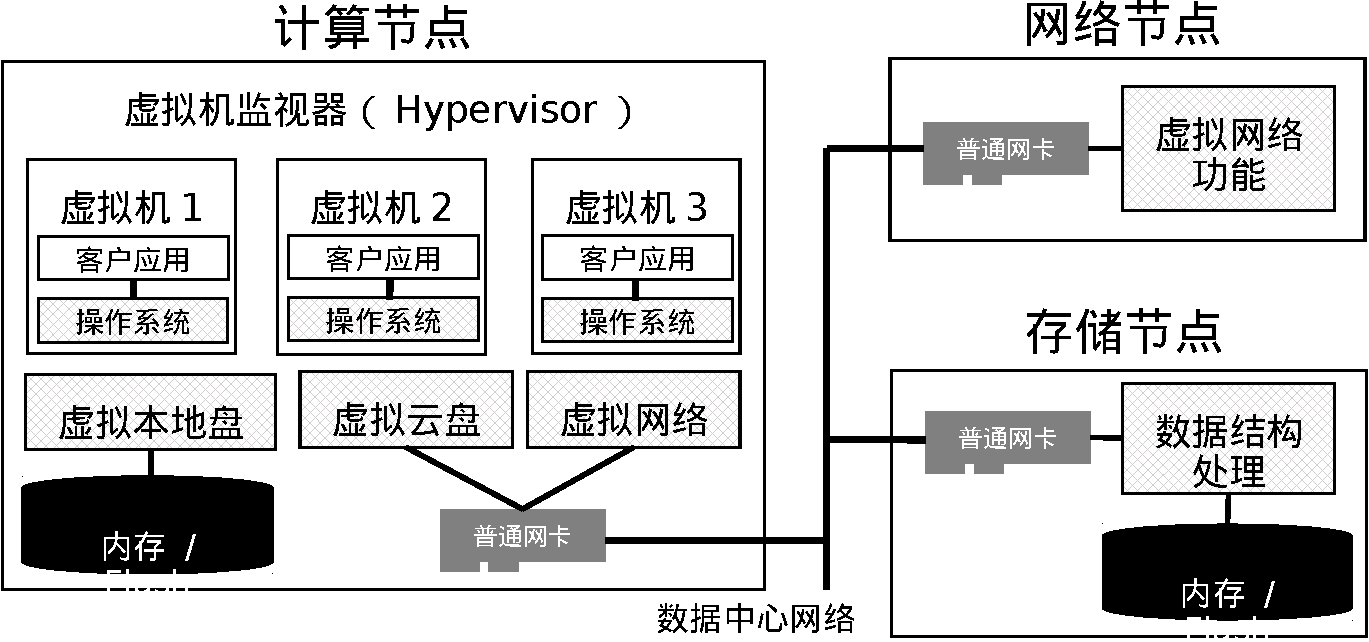
\includegraphics[width=0.8\textwidth]{figures/virt_arch.pdf}
	\caption{虚拟化的数据中心架构。}
	\label{intro:fig:virt-architecture}
\end{figure}


由于云服务的快速迭代,这些虚拟化的网络、存储功能还需要灵活性、可编程性和可调试性,传统上往往用运行在通用处理器上的软件实现。除了虚拟化开销,传统操作系统的开销也不容忽视。这些图 \ref{intro:fig:virt-architecture} 中蓝色方框所示的软件开销被称为 ``数据中心税''(data center tax) \cite{barroso2009datacenter,barroso2013datacenter,barroso2017attack,barroso2018datacenter}。
在网络、存储、定制化计算硬件越来越快的趋势下,数据中心税不仅浪费了大量的 CPU 资源,还导致应用程序无法充分利用硬件的性能。
例如,我们将在第 \ref{chapter:clicknp} 章看到,计算节点需要占用 20\% 左右的 CPU 用来实现网络和存储虚拟化,而计算节点的虚拟网络和网络节点的网络功能都会增加数十乃至上千微秒的延迟。作为比较,数据中心网络本身的延迟只有数微秒至数十微秒,虚拟化增加的延迟比网络本身的延迟还高。
我们也将在第 \ref{chapter:kvdirect} 章看到,软件数据结构存储的性能不仅与内存性能相去甚远,甚至连充分利用持久化闪存的性能都困难。
我们还将在第 \ref{chapter:socksdirect} 章看到,应用程序普遍使用操作系统中的套接字原语来进行通信,对于 Web 服务器等通信密集型的应用程序,操作系统占用了 50\% 至 90\% 的 CPU 时间;而且,操作系统实现的套接字原语比硬件提供的远程直接内存访问(RDMA)原语延迟高一个数量级。

综上,通过软硬件结合的全栈优化降低 ``数据中心税'' 对现代数据中心的性能和成本有重要意义,这也是本文研究的课题。





\section{国内外研究现状}

为了降低 ``数据中心税'' 的开销,学术界和工业界提出了很多方案,大致可以分为优化软件、利用新型商用硬件和设计新硬件三类。

\subsection{优化软件}

虚拟网络通常用虚拟交换机软件实现,如 Open vSwitch \cite{pfaff2015design}。
为了提高虚拟网络的性能,并满足可编程性要求,云服务商重新设计了软件虚拟交换机,如微软的 VFP \cite{firestone2017vfp} 和谷歌的 Andromeda \cite{andromeda}。
通过利用 DPDK \cite{dpdk} 等高速网络处理包技术,并使用轮询模式运行 CPU 核,我们可以绕过 OS 网络协议栈来显著降低数据包处理成本。
%SoftNIC \cite{han2015softnic} 提出用软件实现网卡中固化的功能以提高灵活性。
但是,即使是不做任何处理的简单网络数据包转发,每个 CPU 核每秒也只能处理 10 M 至 20 M 个数据包 \cite{martins2014clickos,netbricks},对于 60 M 个数据包每秒的 40 Gbps 线速,仍然需要 3 至 6 个 CPU 核。

为了支持灵活的网络功能,云服务商还部署了软件实现的虚拟网络功能。例如,Ananta \cite {ananta} 是一个部署在微软数据中心的软件负载均衡器,用于提供云规模的负载均衡服务。
为了在一台服务器上支持多种网络功能,RouteBricks \cite {routebricks}、xOMB \cite{anderson2012xomb} 和 COMB \cite{comb} 采用 Click 模块化路由器 \cite{kohler2000click} 的编程模型,把每个网络功能实现成一个 C++ 的类,让每个数据包在一个 CPU 核上依次被各个网络功能处理,即所谓 ``运行到结束(run-to-completion)'' 模型。
这些工作表明,在实际网络功能下,基于多核 x86 CPU 的每台服务器转发数据包的速度可达 10 Gbps,并且可以通过多核和搭建更多网络节点的集群来扩展容量。
为了实现网络功能之间的隔离,NetVM \cite{hwang2015netvm}、ClickOS \cite{martins2014clickos}、HyperSwitch \cite{ram2013hyper}、mSwitch \cite{eisenbud2016maglev} 等工作把每个网络功能放在一个(轻量级)虚拟机里,并让虚拟交换机把数据包依次分发给这些虚拟机处理,即所谓 ``流水线'' 模型。
流水线模型中,数据包在多核之间反复传递,开销较高。
NetBricks \cite{netbricks} 回到了 ``运行到结束'' 模型,但用高级语言实现网络功能,并在编译器和运行框架的层面上保证网络功能之间的隔离性。
NFP \cite{sun2017nfp} 利用多个并行的网络功能流水线提高数据包处理的性能。

为了数据的可靠性、容量的可扩放性和分布式计算中的数据共享,云上的数据一般是存储在分布式存储系统中。
作为一种重要的基础设施,分布式键值存储系统的研究和开发受到性能的驱动。大量分布式KVS基于CPU。为了降低计算成本,Masstree~ \cite {mao2012cache},MemC3~ \cite {fan2013memc3}和libcuckoo~ \cite {li2014algorithmic}优化锁定,缓存,散列和内存分配算法。MICA~ \cite {lim2014mica}将哈希表分区到每个核心,从而完全避免同步。然而,这种方法为偏移的工作负载(skewed workload)引入了 CPU 核之间的不平衡。


内核网络堆栈优化:第一项工作是优化内核TCP / IP堆栈。 FastSocket~ \cite {lin2016scalable},Affinity-Accept~ \cite {pesterev2012improving},FlexSC~ \cite {soares2010flexsc}和零拷贝套接字 \cite {thadani1995efficient,chu1996zero,linux-zero-copy}实现良好的兼容性和隔离性。

MegaPipe~ \cite {han2012megapipe}和StackMap~ \cite {yasukata2016stackmap}提出了新的API来实现零拷贝和改进I / O多路复用,代价是需要修改应用程序。
但是,大量的内核开销仍然存在。
支持零拷贝的挑战是套接字语义,如章节 \ref {socksdirect:subsec:per-byte-overhead}中所述。

用户空间TCP / IP堆栈:第二项工作完全绕过内核TCP / IP堆栈并在用户空间中实现TCP / IP。
在这个类别中,IX~ \cite {belay2017ix}和Arrakis~\cite {peter2016arrakis}是新的操作系统架构,它使用虚拟化来确保安全性和隔离性。 IX利用LwIP~ \cite {dunkels2001design}在用户空间中实现TCP / IP,同时使用内核转发每个数据包以实现性能隔离和QoS。相比之下,Arrakis将QoS卸载到NIC,因此绕过数据平面的内核。
他们使用NIC在同一主机中的应用程序之间转发数据包。
如表 \ref {socksdirect:tab:operation-performance}所示,从CPU到NIC的发夹延迟远远高于核心间缓存迁移延迟。
吞吐量也受到内存映射I / O(MMIO)门铃延迟和PCIe带宽的限制 \cite {neugebauer2018understanding,li2017kv}。

除了这些新的OS体系结构外,许多用户空间套接字在Linux上使用高性能数据包I / O框架,例如Netmap~ \cite {rizzo2012netmap},Intel DPDK~ \cite {dpdk}和PF\_RING \cite {pf-ring},以便直接访问用户空间中的NIC队列。
SandStorm~ \cite {marinos2014network},mTCP~ \cite {jeong2014mtcp},Seastar~ \cite {seastar}和F-Stack~ \cite {fstack}提出了新的API,因此需要修改应用程序。
大多数API更改旨在支持零拷贝,标准API仍然会复制数据。
FaSST~ \cite {kalia2016fasst}和eRPC~ \cite {kalia2018datacenter}提供RPC API而不是套接字。
LibVMA~ \cite {libvma},OpenOnload~ \cite {openonload},DBL~ \cite {dbl}和LOS~ \cite {huang2017high}符合标准套接字API。
用户空间TCP / IP堆栈提供了比Linux更好的性能,但它仍然不接近RDMA和SHM。
一个重要原因是现有的工作都不支持在线程和进程之间共享套接字,导致多线程锁定开销。
不支持套接字共享还导致进程分叉(fork)和容器热迁移(container live migration)中的兼容性问题。
这将在第 \ref{chapter:socksdirect} 中进一步讨论。



\subsection{利用新型商用硬件}


由于大规模 Web 服务、大数据处理、机器学习等应用对计算和网络的性能需求非常迫切,GPU,RDMA……


为了加速软件包处理,以前的工作已经提出使用GPU \cite {packetshader},专用网络处理器(NP)\cite {cavium,netronome} 和硬件交换机 \cite {duet}。
GPU主要用于图形处理,最近扩展到具有海量数据并行性的其他应用程序。 GPU更适合批量操作。 PacketShader \cite {packetshader},表明使用GPU可以实现40Gbps的分组交换速度。
但是,批量操作会导致高延迟。
例如,\cite {packetshader}中报告的转发延迟约为$200 \mu{}s$。



为了摆脱操作系统内核的开销, \cite {rizzo2012netmap,intel2014data}直接轮询来自NIC的网络数据包,并且\cite {jeong2014mtcp,marinos2014network}使用用户空间轻量级网络堆栈处理它们。
键值存储系统 \cite {kapoor2012chronos,ousterhout2010case,ousterhout2015ramcloud,lim2014mica,li2016full}受益于这种高性能优化。
作为朝着这个方向迈出的又一步,最近的作品\cite {infiniband2000infiniband,kalia2014using,kalia2016design,kalia2014using,kalia2016design}利用RDMA NIC的基于硬件的网络堆栈,使用双面RDMA作为KVS客户端和服务器之间的RPC机制进一步提高每核吞吐量并减少延迟。尽管如此,这些系统仍受CPU限制(\S \ref {kvdirect:sec:state-of-the-art-kvs})。

另一种不同的方法是利用单侧RDMA。 Pilaf~ \cite {mitchell2013using}和FaRM~ \cite {dragojevic2014farm}采用单向RDMA读取进行GET操作,FaRM实现了使网络饱和的吞吐量。 Nessie~ \cite {szepesi2014designing},DrTM~ \cite {wei2015fast},DrTM + R~ \cite {chen2016fast}和FaSST~ \cite {kalia2016fasst}利用分布式事务来实现单向RDMA的GET和PUT。但是,PUT操作的性能受到一致性保证的不可避免的同步开销的影响,受到RDMA原语的限制 \cite {kalia2016design}。此外,客户端CPU涉及KV处理,将每个核心的吞吐量限制在客户端的大约10~Mops。
相比之下,本文将RDMA原语扩展到键值操作,同时保证服务器端的一致性,使KVS客户端完全透明,同时实现高吞吐量和低延迟,即使对于PUT操作也是如此。

二级索引是通过其他键检索数据的重要功能
比数据存储系统中的主键 \cite {escriva2012hyperdex,kejriwal2016slik}。 SLIK~ \cite {kejriwal2016slik}在键值存储系统中使用B +树算法支持多个二级密钥。探索如何支持二级索引以帮助本文迈向通用数据存储系统将会很有趣。 SwitchKV~ \cite {li2016fast}利用基于内容的路由将请求路由到基于缓存密钥的后端节点,NetCache~ \cite {netcache-sosp17}进一步将KV缓存在交换机中。这种负载平衡和缓存也将使我们的系统受益。
Eris~ \cite {eris}利用网络序列发生器来实现高效的分布式事务,这可以为客户端同步的单侧RDMA方法带来新的生命。

存储虚拟化……


第三行研究将套接字系统的一部分卸载到NIC硬件上。
TCP卸载引擎(TOE) \cite {tcp-chimney-offload}将部分或完整的TCP / IP堆栈卸载到NIC,但它们仅在专用区域中起飞(例如iSCSI HBA~ \cite {iscsi-hba})和无状态卸载(例如校验和,流动转向和LSO / LRO~ \cite {lsolro})。
由于数据中心的硬件趋势和应用需求,\emph {stateful}卸载的故事近年来有所不同 \cite {chuanxiong-rdma-keynote}。
因此,RDMA~ \cite {infiniband2000infiniband}在生产数据中心中广泛使用 \cite {guo2016rdma}。
与基于软件的TCP / IP网络堆栈相比,RDMA使用硬件卸载来提供超低延迟和接近零的CPU开销。
要使套接字应用程序能够使用RDMA,RSocket~ \cite {rsockets},SDP~ \cite {socketsdirect}和UNH EXS~ \cite {russell2008extended}将套接字操作转换为RDMA谓词。
它们具有相似的设计,而RSocket是最活跃的设计。
FreeFlow~ \cite {nsdi19freeflow}虚拟化容器覆盖网络的RDMA NIC,它利用SHM进行主机内部和RDMA进行主机间通信。
FreeFlow使用RSocket将套接字转换为RDMA。


应用层:存储复制,数据库事务

GPS: Google Spanner

可编程交换机

Recent years witness a trend of co-designing consensus protocols with data center network.
The key idea is to provide FIFO and total ordering in the network, going a step further than best-effort ordering in Fast Paxos~\cite{lamport2006fast,kemme1999processing,moraru2013there,pedone1998optimistic}.
Speculative Paxos~\cite{ports2015designing} and NOPaxos~\cite{li2016just} use a switch as a centralized sequencer or serialization point.
NetPaxos~\cite{dang2015netpaxos,dang2016paxos} and \cite{dang2016network} implement Paxos in switches.
Eris~\cite{eris} proposes in-network concurrency control using switch as a centralized sequencer, which is a scalability bottleneck.
NetChain~\cite{jin2018netchain} is a strongly-consistent fault-tolerant key-value store in switches, but the switch has very limited storage capacity.

HyperLoop nsdi


\subsection{设计新硬件}

为深度学习设计新硬件,TPU……

随着通用处理器的性能提升遇到了瓶颈,各大云服务商开始探索使用定制化硬件来 ``减税降负'',也就是把数据中心的虚拟化、操作系统和高层抽象的开销从通用处理器转移到定制化硬件上。
使用定制化硬件并不是在硬件中原样实现已有的软件,而是对已有软件进行重构,划分出数据面和控制面,数据面优化后在硬件中实现,控制面则留在软件上。
采用新硬件的方案尽管性能较高,但不仅需要新硬件的资产和运营成本,还需要软硬件协同设计的开发成本,往往比优化软件的开发成本更高。
因此,不是所有软件都适合用硬件来加速,需要权衡成本和收益。


虽然软件实现的虚拟交换机和网络功能可以使用更多数量的 CPU 核和更大的网络节点集群来支持更高的性能,但这样做会增加相当大的资产和运营成本 \cite {ananta,duet}。
云服务商在 IaaS 业务中的盈利能力是客户为虚拟机支付的价格与托管虚拟机的成本之间的差异。
由于每台服务器的资产和运营成本在上架部署时就已基本确定,因此降低托管虚拟机成本的最佳方法是在每台计算节点服务器上打包更多的客户虚拟机。
目前,物理 CPU 核(2 个超线程)的售价为 0.1 美元/小时左右,亦即最大潜在收入约为 900 美元/年。
在数据中心,服务器通常服役 3 到 5 年,因此一个物理 CPU 核在服务器生命周期内的售价最高可达 4500 美元 \cite{smartnic}。
即使考虑到总有一部分 CPU 核没有被售出,并且云经常为大客户提供折扣,与专用硬件相比,即使专门分配一个物理 CPU 核用于虚拟网络也是相当昂贵的。
为了尽可能减少计算节点上用于虚拟网络的 CPU 核,以微软 Azure 云为代表的云服务商在数据中心的每台服务器上部署了一块可编程网卡,用以加速计算节点上的虚拟网络 \cite{smartnic}。
为了在提供高性能的同时保持一定的可编程性和灵活性,业界提出了专用芯片(ASIC)、网络处理器(Network Processor)、多核通用处理器片上系统(SoC)、现场可编程门阵列(FPGA)等可编程网卡架构。

学术界也提出了多种基于专用芯片的网卡架构,如 FlexNIC \cite{kaufmann2016high}。
基于专用芯片的柜顶交换机和可编程网卡灵活性较差,而基于通用处理器的可编程网卡和 GPU 有一定的性能局限性。
FPGA 在性能和灵活性间达到了折中,因此微软采用了基于 FPGA 的可编程网卡 \cite{putnam2014reconfigurable}。

AWS Nitro …… 国内 ……



FPGA是一项成熟的技术,最近已经部署用于加速数据中心服务,包括网络功能 \cite {putnam2014reconfigurable,smartnic,rubow2010chimpp,lavasani2012compiling}。
众所周知,FPGA的可编程性很低,有丰富的前人工作提供了高级编程抽象 \cite {bluespec,auerbach2010lime,bacon2013fpga,singh2011implementing,bachrach2012chisel,wester2015transformation}。
Gorilla \cite {lavasani2012compiling} 为FPGA上的数据包交换提出了一种领域特定的高级语言。
然而,Chimpp \cite {rubow2010chimpp} 试图将Click模型引入HDL来开发模块化路由器。

Click2NetFPGA~\cite {Click2NetFPGA}通过直接将Click模块化路由器\cite {kohler2000click}程序编译到FPGA中来提供模块化架构。
然而,\cite {Click2NetFPGA}的性能比我们在本文中报告的要低得多(两个数量级),因为它们的系统设计存在几个瓶颈(例如,内存和数据包I / O),它们也是 错过几个重要的优化以确保完全流水线处理(如\S \ref {clicknp:sec:optimization}中所述)。
此外,\cite {Click2NetFPGA}不支持FPGA / CPU联合处理,因此无法在数据平面运行时更新配置或读取状态。




作为一种灵活且可定制的硬件,FPGA现已广泛部署在数据中心规模 \cite {putnam2014reconfigurable,caulfield2016cloud}中,并且针对可编程性进行了大幅改进 \cite {bacon2013fpga,li2016clicknp}。一些早期的工作已探索在FPGA上构建KVS。但是其中一些是不实用的,限制片上数据存储(大约几MB内存) \cite {liang16fpl}或板载DRAM(通常是8GB内存) \cite {istvan2013flexible,chalamalasetti2013fpga,istvan2015hash}。
\cite {blott2015scaling}专注于提高系统容量而不是吞吐量,并采用SSD作为板载DRAM的二级存储。
\cite {liang16fpl,chalamalasetti2013fpga}限制它们在固定大小键值对中的使用,这只能用于特殊用途,而不是一般的键值存储。
\cite {blott13hotcloud,lavasani2014fpga}使用主机DRAM存储哈希表,而\cite {tokusashi2016multilevel}使用NIC DRAM作为主机DRAM的缓存,但它们没有针对网络和PCIe DMA带宽进行优化,导致性能不佳。
本文充分利用了NIC DRAM和主机DRAM,使我们基于FPGA的键值存储系统通用,并且能够进行大规模部署。此外,我们精心的硬件和软件协同设计,以及对PCIe和网络的优化,将性能推向了物理限制,推进了最先进的解决方案。


传统上,FPGA使用Verilog、VHDL等硬件描述语言编程。众所周知,硬件描述语言难以调试、编写和修改,给软件人员使用FPGA带来了很大挑战。

为了提高FPGA的开发效率,FPGA厂商提供了高层次综合(HLS)工具~\cite{vivado,intel-hls},可以把C代码编译成硬件模块。学术界提出了 Chisel \cite{bachrach2012chisel} 等。但这些工具只是硬件开发工具链的补充,程序员仍然需要手动将从C语言生成的硬件模块插入到HDL项目中,且FPGA与主机CPU之间的通信也需要自行处理。这样的模型仍然不足以让软件开发人员使用FPGA。

近年来,为了让软件开发人员使用FPGA,FPGA厂商提出了基于OpenCL的编程工具链~\cite{aoc,sdaccel},提供了类似GPU的编程模型。软件开发人员可以把用OpenCL语言编写的核(kernel)卸载到FPGA上。但是,这种方法中多个并行执行的核间需要通过板上共享内存进行通信,而FPGA上的DRAM共享内存吞吐量和延迟都不理想,共享内存还会成为通信瓶颈。其次,FPGA与CPU之间的通信模型是类似GPU的批处理模型,这使得处理延迟较高(约1毫秒),不适用于需要微秒级延迟的网络数据包处理。







\section{本文的研究内容和贡献}


本文旨在探索基于可编程网卡的高性能数据中心系统。本文提出一个基于 FPGA 可编程网卡,对云计算数据中心计算、网络、存储节点实现全栈加速的系统。如图 \ref{intro:fig:accel-arch} 所示,我们把计算、网络、存储节点上的普通网卡替换为可编程网卡。我们在计算节点上实现了虚拟网卡和虚拟网络,虚拟本地存储和云存储,以及轻量级用户态运行库和硬件传输协议相结合的通信原语,替代了图 \ref{intro:fig:virt-architecture} 中的软件虚拟化服务和操作系统网络协议栈。我们利用数据面与控制面分离的思想,在网络节点上实现虚拟网络功能,在存储节点上实现数据结构处理,用可编程网卡提高了数据面性能,并保留原有软件控制面的灵活性。


\begin{figure}[htbp]
	\centering
	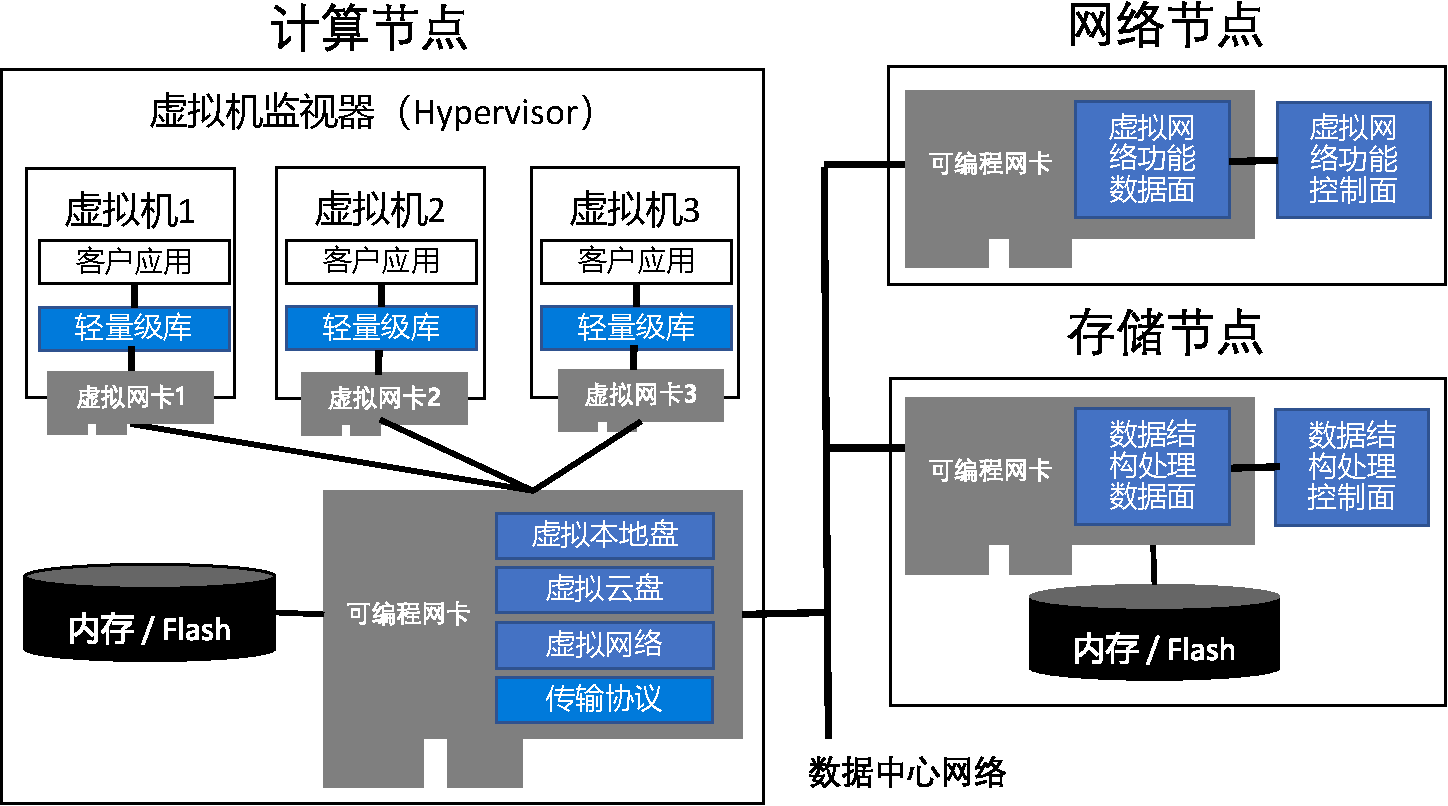
\includegraphics[width=0.8\textwidth]{figures/accel_arch.pdf}
	\caption{基于可编程网卡的数据中心系统总体架构。}
	\label{intro:fig:accel-arch}
\end{figure}

首先,本文提出用可编程网卡加速云计算中的虚拟网络功能。我们提出了首个在商用服务器中用 FPGA 加速的高灵活性、高性能网络功能处理平台 ClickNP。众所周知,FPGA 编程对软件工程师很不友好。为了简化 FPGA 编程,我们设计了类 C 的 ClickNP 语言和模块化的编程模型,并开发了一系列优化技术,以充分利用 FPGA 的海量并行性。我们实现了 ClickNP 开发工具链,可以与多种商用高层次综合工具集成。我们基于 ClickNP 设计和实现了 200 多个网络元件,并用这些元件组建起多种网络功能。相比基于 CPU 的软件网络功能,ClickNP 的吞吐量提高了 10 倍,延迟降低到 1/10;且具有可忽略的 CPU 开销,可以为云计算中的每个计算节点节约 20\% 的 CPU 核。

其次,本文提出用可编程网卡加速远程数据结构访问。键值存储是最常用的基本数据结构之一,也是很多数据中心内的关键分布式系统组件。我们基于 ClickNP 编程框架,设计实现了一个高性能内存键值存储系统 KV-Direct,在服务器端绕过 CPU,用可编程网卡通过 PCIe 直接访问主机内存。我们把单边 RDMA 的内存操作语义扩展到键值操作语义,解决了单边 RDMA 操作数据结构时通信和同步开销高的问题。我们还利用 FPGA 可重配置的特性,允许用户实现更复杂的数据结构。面对网卡与主机内存之间 PCIe 带宽较低、延迟较高的性能挑战,我们设计了哈希表、内存分配器、乱序执行引擎、负载均衡和缓存、向量操作等一系列性能优化,实现了 10 倍于 CPU 的能耗效率和微秒级的延迟,实现了首个单机性能达到 10 亿次每秒的通用键值存储系统。

最后,本文提出用可编程网卡和用户态运行库相结合的方法为应用程序提供系统原语,从而绕过操作系统内核。套接字是操作系统提供的最常用的通信原语。我们设计实现了一个用户态套接字系统 SocksDirect,与现有应用程序完全兼容,能实现接近硬件极限的吞吐量和延迟,多核性能具有可扩放性,并在高并发负载下保持高性能。我们分别使用共享内存和 RDMA 实现主机内和主机间的通信。为了支持高并发连接数,我们基于 KV-Direct 实现了一个 RDMA 可编程网卡。我们消除了线程间同步、缓冲区管理、大数据拷贝、进程唤醒等一系列开销。SocksDirect 相比 Linux 提升了 7 至 20 倍吞吐量,降低延迟到 1/17 至 1/35,并将 Web 服务器的 HTTP 延迟降低到 1/5.5。


\section{论文结构安排}

本论文的内容结构安排如下:
第 1 章为绪论。
第 2 章介绍数据中心的背景知识、虚拟化架构和相关工作,分析硬件的发展趋势,对可编程网卡的架构进行分类,并调研可编程网卡在数据中心的应用。
第 3 章提出基于可编程网卡的数据中心系统架构。
第 4 章提出用可编程网卡加速云计算中的虚拟网络功能。为了简化 FPGA 编程,提出首个适用于高速网络数据包处理、基于高级语言的模块化 FPGA 编程框架 ClickNP。
第 5 章提出用可编程网卡加速远程数据结构访问,并设计实现一个高性能内存键值存储系统 KV-Direct。
第 6 章提出用可编程网卡和用户态运行库相结合的方法为应用程序提供操作系统原语,并设计实现一个用户态套接字系统 SocksDirect。
第 7 章总结全文并展望未来研究方向。